\pagenumbering{Roman}
\begin{annexes}{A. Vistas del sistema}
    % \setcounter{figure}{0}
    % Game UIs:
    \begin{figure}[!ht]
        \centering
        \subfigure[Error: Correo incorrecto]{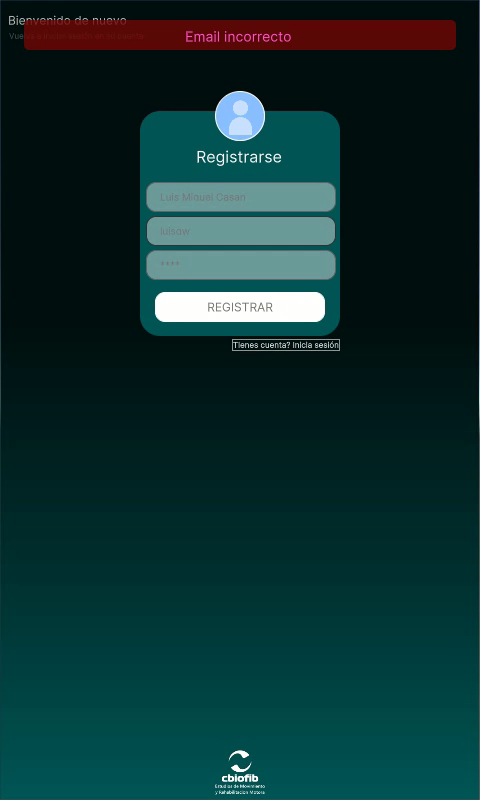
\includegraphics[scale=0.28]{images/ui/ui0.png}}
        \subfigure[Error: Usuario existente]{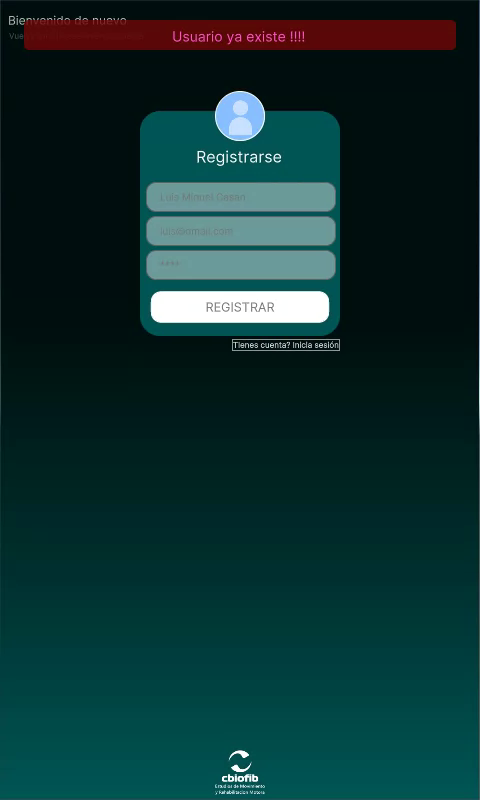
\includegraphics[scale=0.28]{images/ui/ui1.png}}
        \subfigure[Error: Contraseña incorrecta]{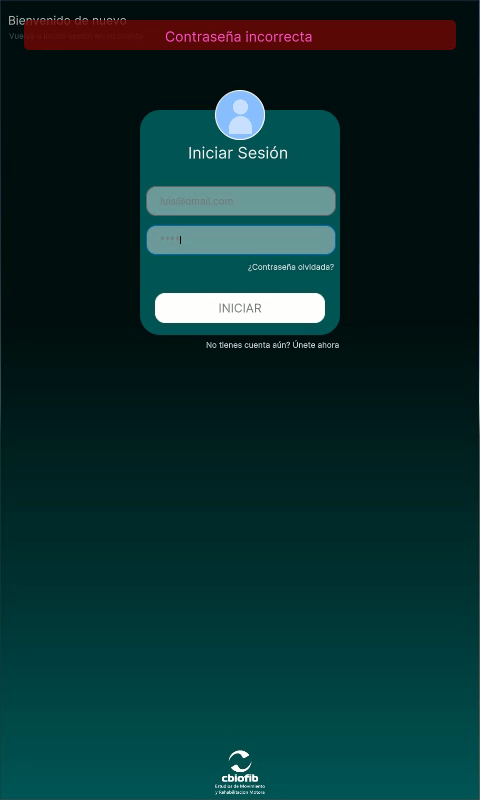
\includegraphics[scale=0.28]{images/ui/ui5.png}}
        \caption{Notificación de errores en la sesión de inicio.}
        \label{annex: 1}
    \end{figure}

    \begin{figure}[!ht]
        \centering
        \subfigure[Inicio de sesión]{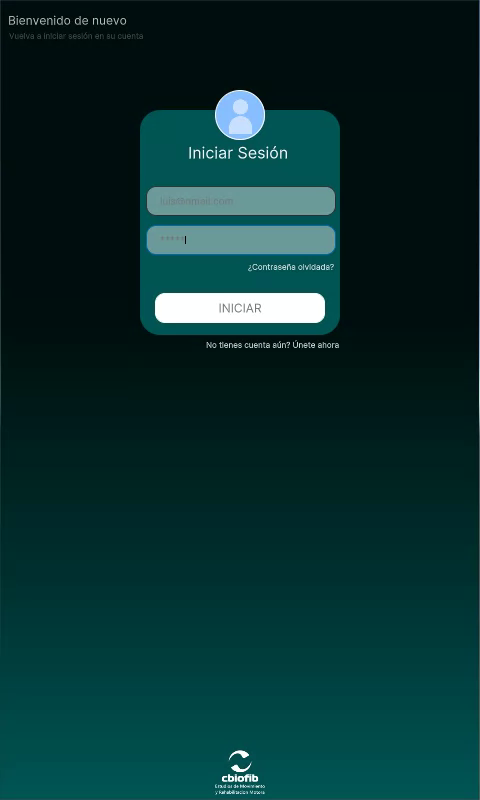
\includegraphics[scale=0.28]{images/ui/ui4.png}}
        \subfigure[Registro de usuario]{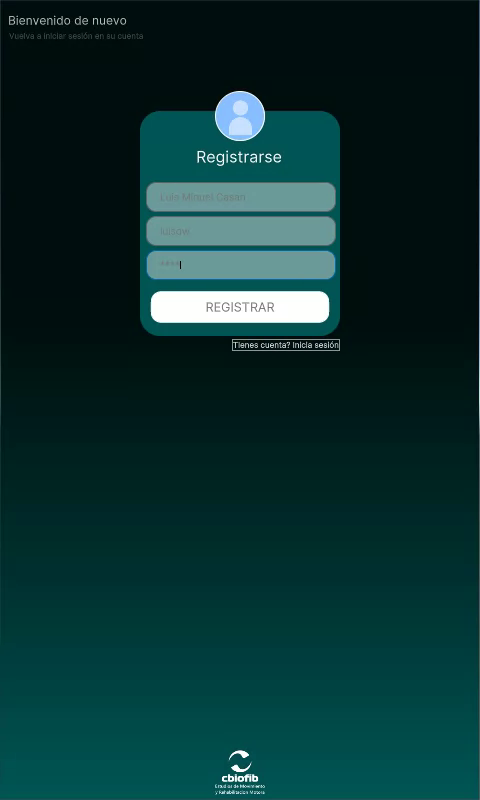
\includegraphics[scale=0.28]{images/ui/ui2.png}}
        \caption{Vistas de la sesión de inicio.}
        \label{annex: 2}
    \end{figure}

    \begin{figure}[!ht]
        \centering
        \subfigure[Interfaz modalidad ligero]{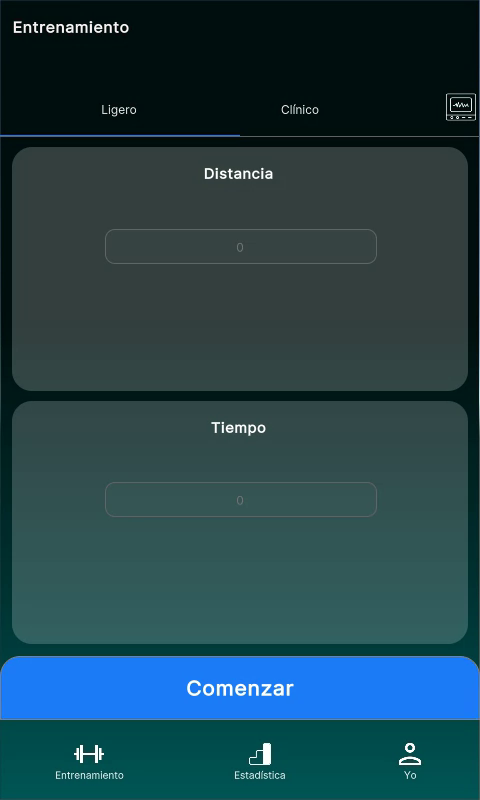
\includegraphics[scale=0.28]{images/ui/ui6.png}}
        \subfigure[Interfaz modalidad clínico]{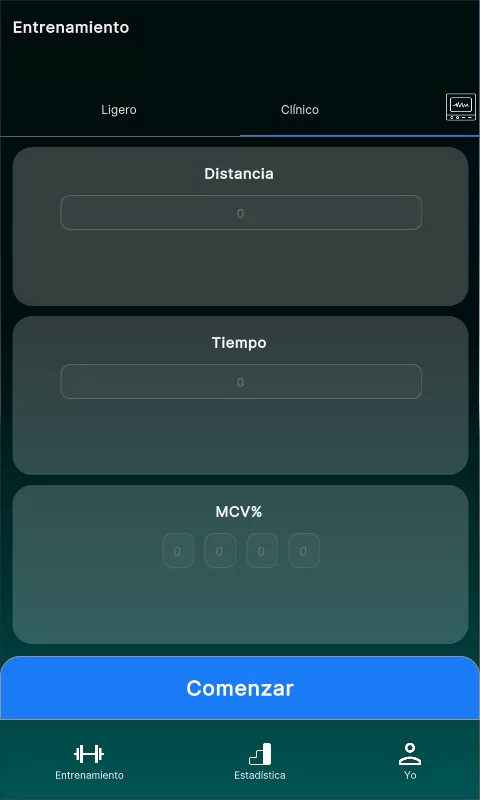
\includegraphics[scale=0.28]{images/ui/ui7.png}}
        \subfigure[Interfaz de calibración]{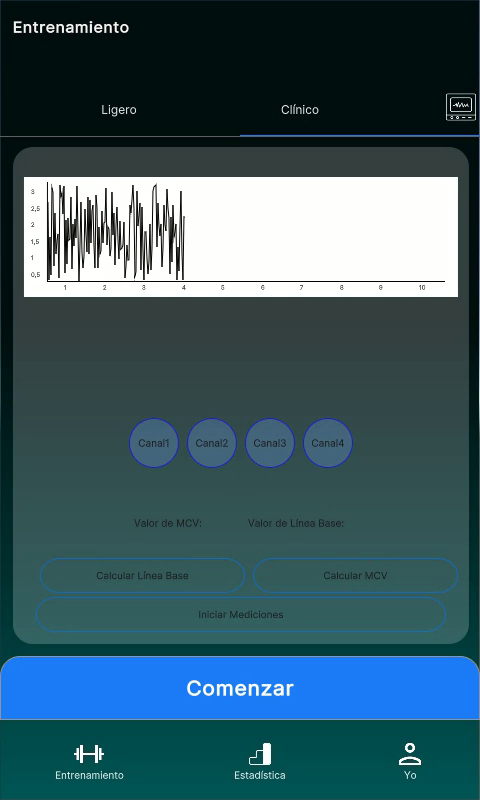
\includegraphics[scale=0.28]{images/ui/ui13.png}}
        \caption{Vistas de la sesión de entrenamiento.}
        \label{annex: 3}
    \end{figure}

    \begin{figure}[!ht]
        \centering
        \subfigure[Configuración de la sesión]{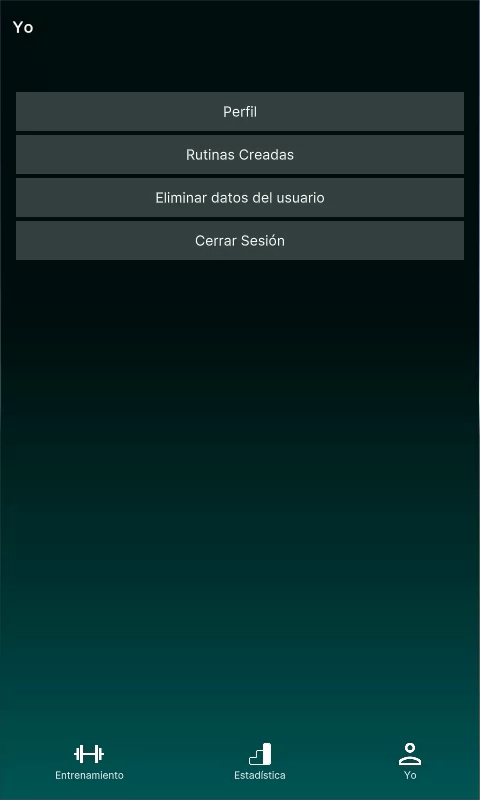
\includegraphics[scale=0.28]{images/ui/ui9.png}}
        \subfigure[Gestionar cuenta de usuario]{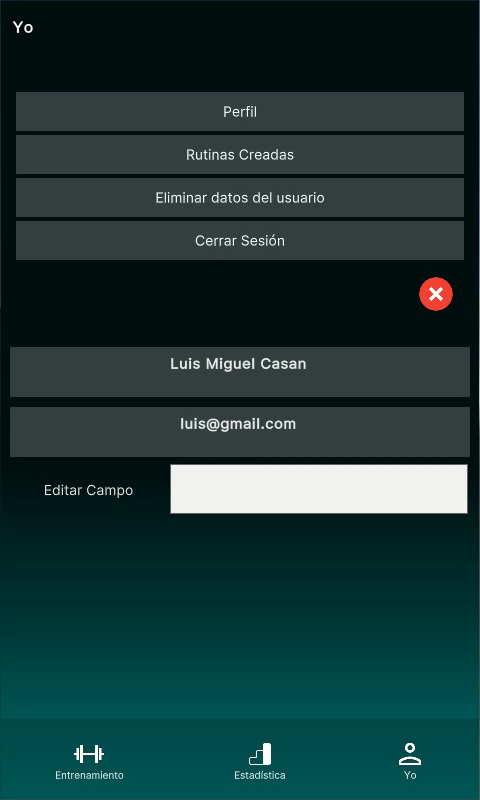
\includegraphics[scale=0.28]{images/ui/ui10.png}}
        \subfigure[Rutinas creadas]{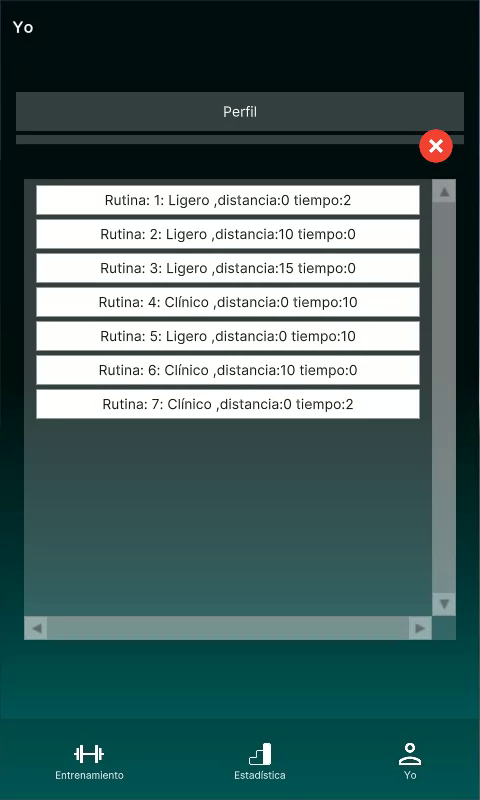
\includegraphics[scale=0.28]{images/ui/ui12.png}}
        \caption{Vistas de la sesión de configuración.}
        \label{annex: 4}
    \end{figure}

    \begin{figure}[!ht]
        \centering
        \subfigure[Gráficos estadísticos]{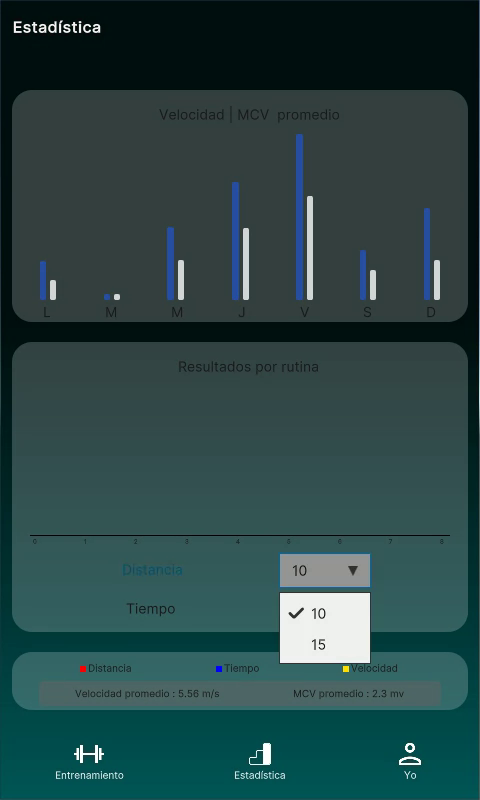
\includegraphics[scale=0.28]{images/ui/ui14.png}}
        \subfigure[Gráficos estadísticos]{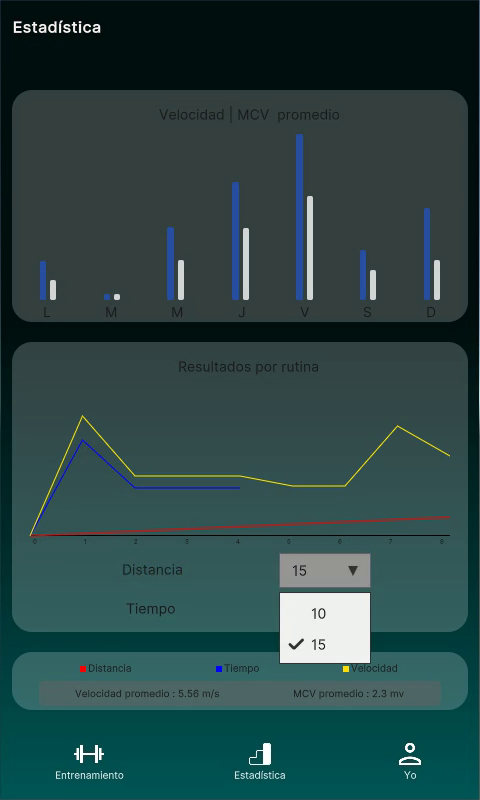
\includegraphics[scale=0.28]{images/ui/ui15.png}}
        \caption{Vistas de la sesión de estadística.}
        \label{annex: 5}
    \end{figure}

    \begin{figure}[!ht]
        \centering
        \subfigure[Modalidad de entrenamiento ligero]{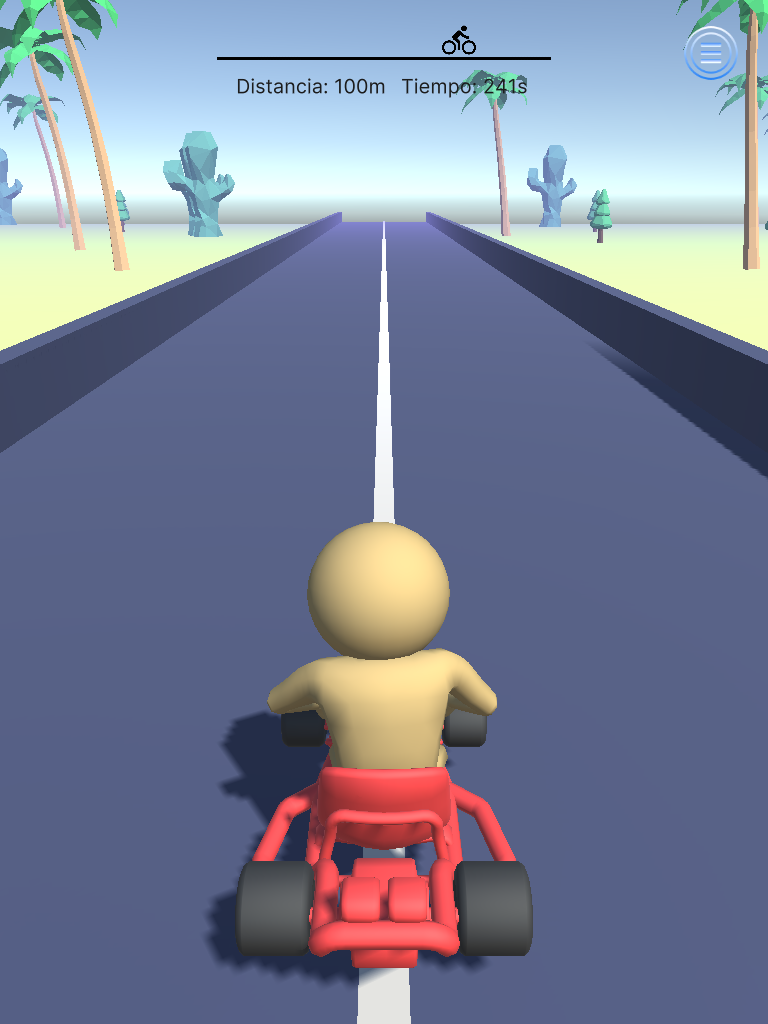
\includegraphics[scale=0.22]{images/ui/lite-modality.png}}
        \subfigure[Modalidad de entrenamiento clínico]{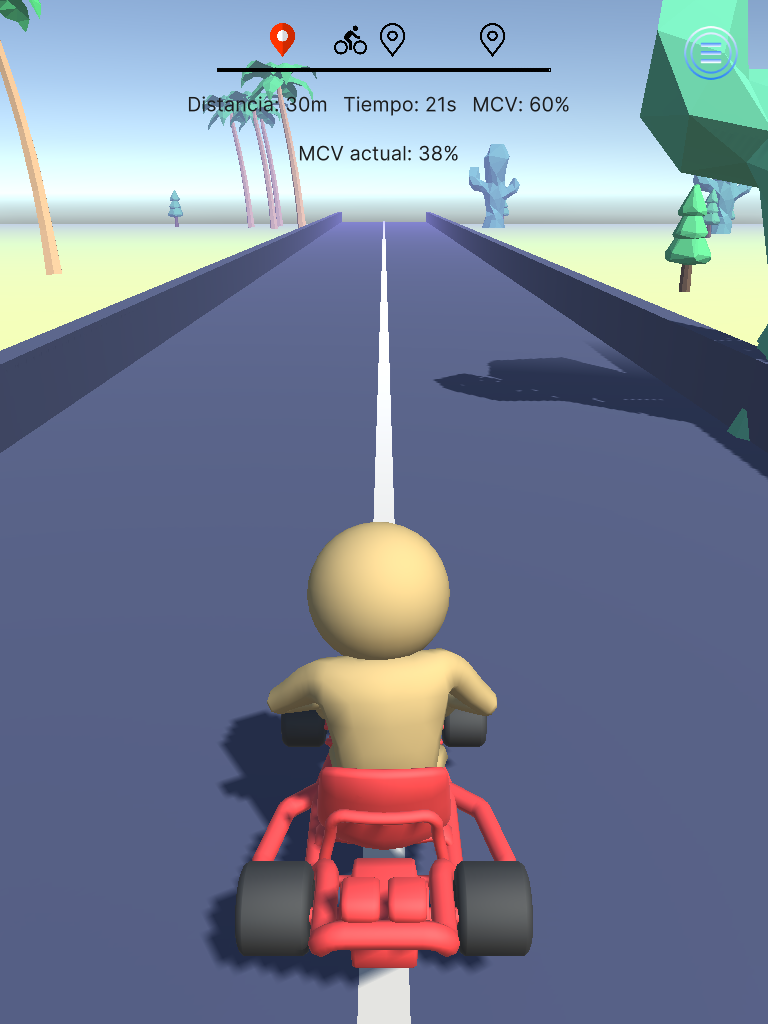
\includegraphics[scale=0.22]{images/ui/clinic-modality.png}}
        \caption{Vistas de las escenas del juego.}
        \label{annex: 6}
    \end{figure}

\end{annexes}